\section{Figure Examples}

This statement automatically references the figure below using its label: Figure \ref{fig:example}.

%------------------------------------------------

\begin{marginfigure} % Use the marginfigure environment for figures to be output to the margin
	
\includegraphics[width=\linewidth]{placeholder.jpg}
	\caption{Margin figure caption.}
\end{marginfigure}

%------------------------------------------------

\begin{figure}[H] % [H] forces the figure to be output where it is defined in the code (it suppresses floating)
	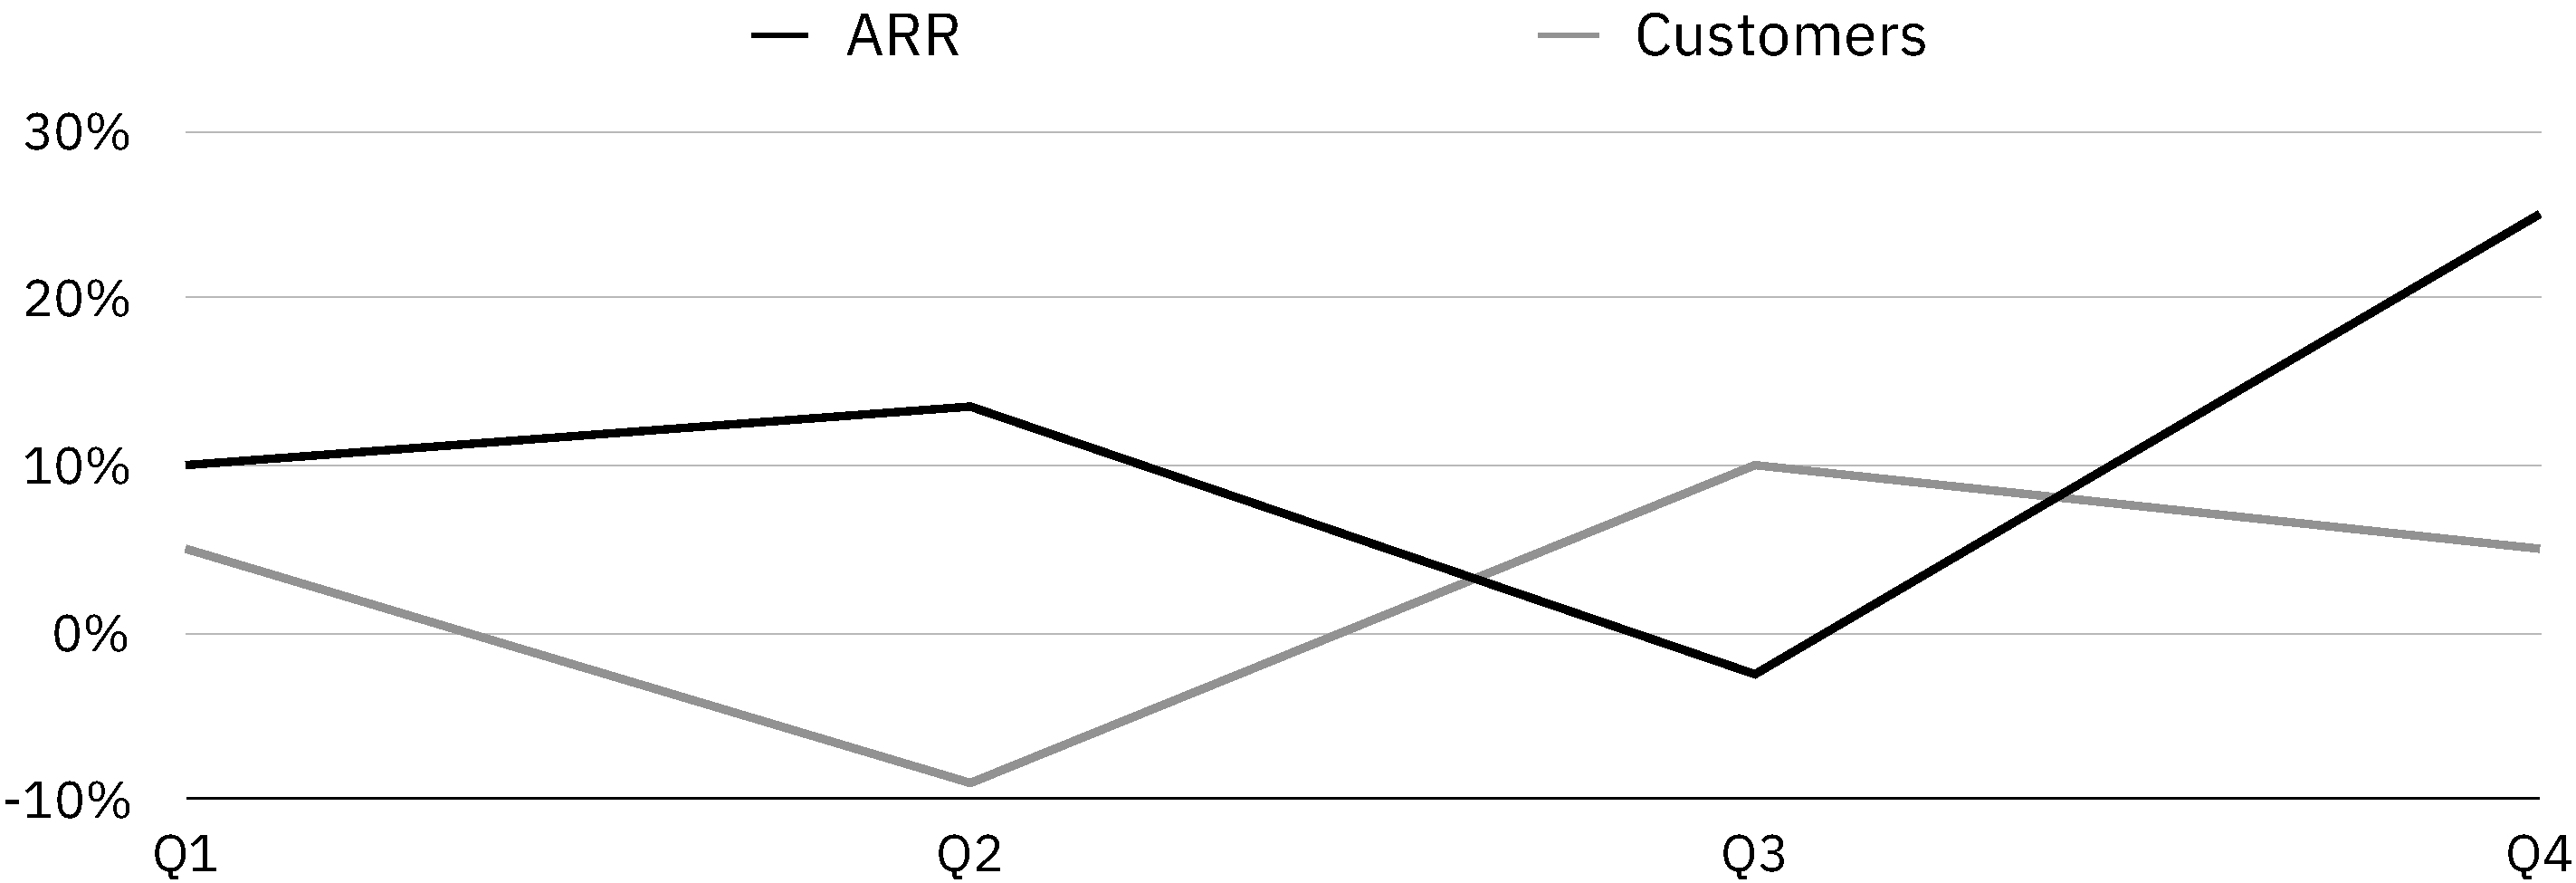
\includegraphics[width=\linewidth]{ARR.pdf}
	\caption{Text block figure caption.}
	\label{fig:example} % Label for referencing this figure in the text automatically
\end{figure}

%------------------------------------------------

\begin{figure*} % Use the figure* environment for full width figures
	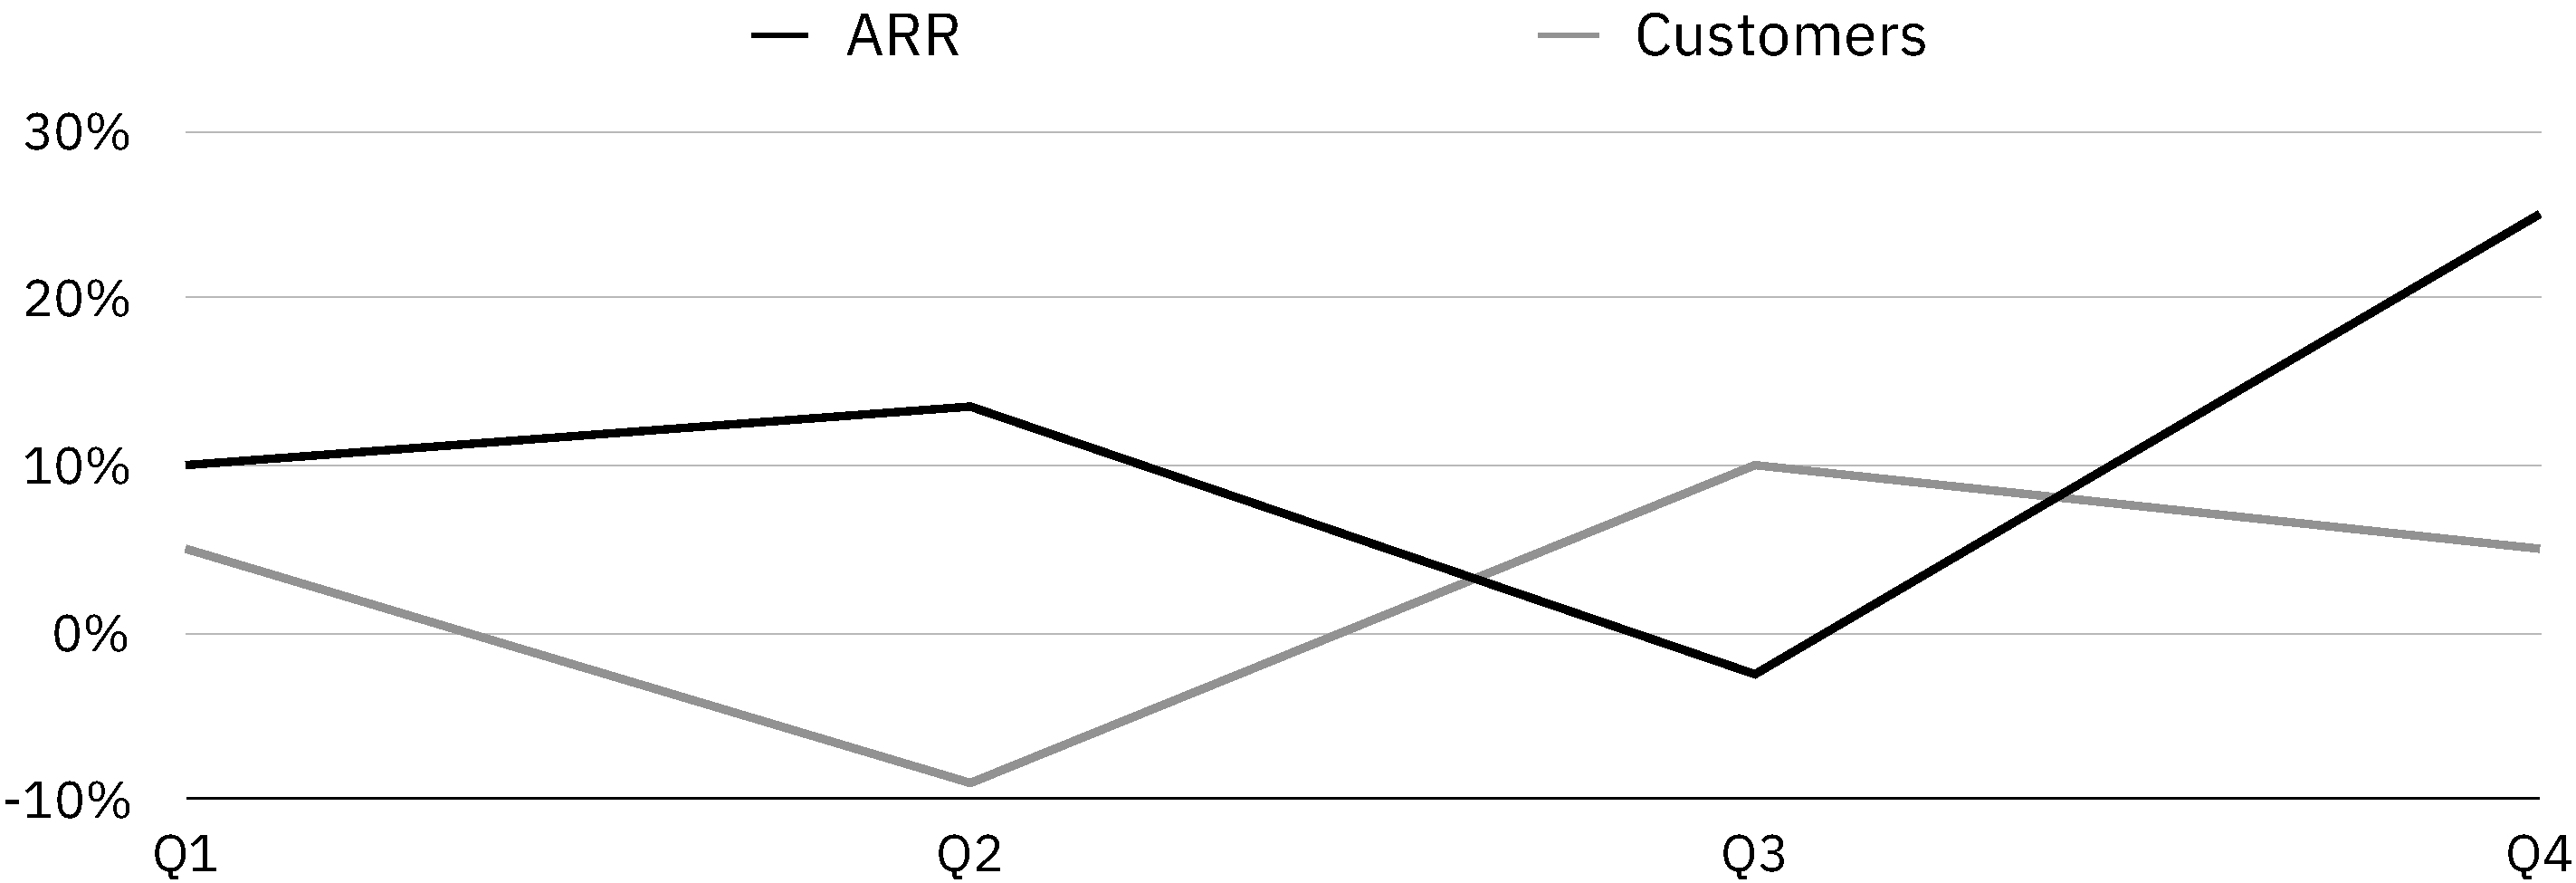
\includegraphics[width=\linewidth]{ARR.pdf}
	\caption{Full width figure caption.}
\end{figure*}